%!TEX root =  main.tex


\section{Our approach}
In this section, we formally describe our \BertMWE approach.
We will start by formally describing our modeling framework in a probabilistic setting, 
and then introduce our approach for modeling the posterior distribution, 
and finally, produce the approximate inference procedure
and discuss some details on how it's implemented in deep transformer network.


\begin{figure}[tb]
    \centering
    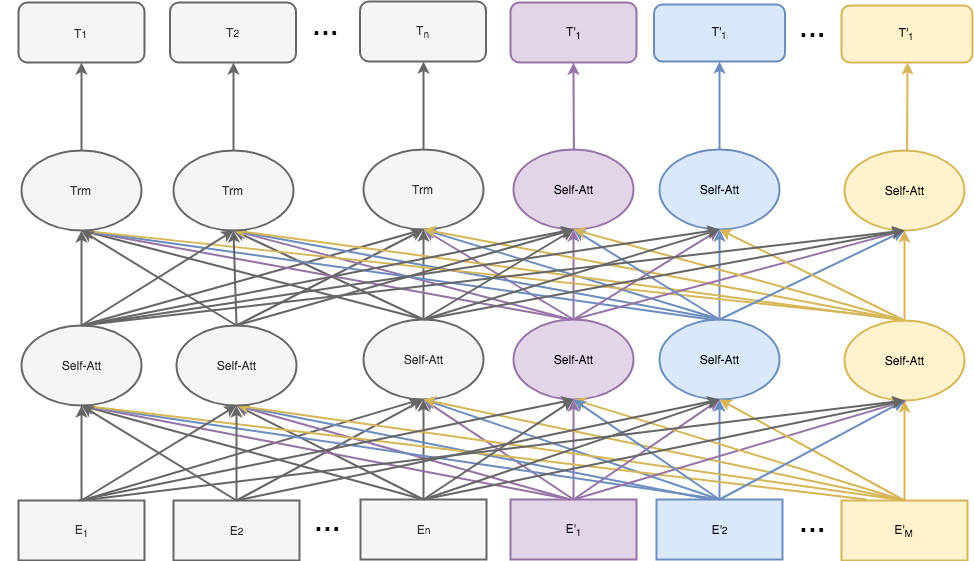
\includegraphics[width=0.95\linewidth]{fig/architecture.png}
    \vspace{20pt}
    \caption{\BertMWE architecture illustration. Grey nodes denotes the original self attention network. Nodes colored in purple, blue and yellow denotes the additional blocks corresponding to specific MWEs.}
    \vspace{10pt}
    \label{fig:variational}
\end{figure}


\subsection{Architecture overview}\label{sec:arch-overview}
In this work we assume that each input text instance are represented as a sequence of tokens $(w_1, ..., w_n)$,
and in addition, there are a set of candidate multi-world expressions $(w'_1, ..., w'_m)$, each corresponds to a span in the original token sequence, with starting index $(st_1, ..., st_m)$, and ending index $(end_1, ..., end_m)$. 

In a typical self-attention network such as the original Bert model \cite{devlin2018bert}, the first step is to transform the input sequence into an unordered set, 
and the original position information is captured using the position embedding mechanism \cite{vaswani2017attention}. Specifically, the  input will be represented in the form of a permutation invariant set $\{u_1, ..., u_n\}$, where each element $u_i=(w_i, pos_i)$ include both the token $w_i$ and its position $pos_i$, which equals to its index in the original sequence $i$.

As illustrated in \autoref{fig:variational}, each element in the input then goes through the embedding layer and are represented as a set of permutation invariant embeddings vectors $\{E_1, ..., E_n\}$, 
\cite{vaswani2017attention}, 
which then goes through a few numbers of inter-connected self-attention layers to be transformed into the final representation, 
$\{T_1, ..., T_n\}$ to be used for specific tasks, such as sequence labeling and classification \cite{devlin2018bert}.

We exploit the crucial observation that input to the downstream self attention network are presented as an unordered set, with the original ordering in the sequence encoded as position embedding,
and proprose an \textit{homogeneous injection} approach to incorporate the MWEs into the network, by feeding the set of MWEs along with the original unordered set to the network, with their position encoded analogously.


Specifically, given a set of candidate multi-world expressions $(w'_1, ..., w'_m)$, 
we will similarly transform them into a set of candidate multi-world expressions $(u'_1, ..., u'_m)$, where each element $u_i=(w'_i, pos'_i)$ includes the MWE $w'_i$ and its location, which is derived as a function of the span location $f(st_i, end_i)$ in the original sequence $pos'_i$ \footnote{in this work we instantiate it as the average function $f(st_i, end_i) = \lceil \frac{st_i, end_i}{2} \rceil $}.
Then, analagously, we embed the multi-world expressions $(u'_1, ..., u'_m)$ into embeddings vectors $\{E'_1, ..., E'_m\}$.
As shown in \autoref{fig:variational}, the embedding vectors $\{E'_1, ..., E'_m\}$ are concatenated with the original vectors, and the newly concatenated set vectors 
$\{E_1, ..., E_n, E'_1, ..., E'_m\}$ are in the exact same form of the original input and fed to the exact same model as before.

The challenge with this approach, however, is that we do not know apriori how many of the candidate MWEs are truly non-compositional and  important for downstream prediction tasks:
Simply adding all of them into the original tokens' embedding would potentially introduce a large amount of noise to the data and obfuscate the original inputs. Blindly ignoring some candidates might miss important non-compositionality information.
we need a way to distinguish good from the bad, and dynamically infer the non-compositionality, along with the set of parameters contained in the deep self-attention networks architecture.

We formulate this using a principled Bayesian probabilistic framework. 
Given a dataset $\mathcalD$ containing a set of $N$ observations of tuples $(x,y)$,  $x$ is the input text and $y$ is the target labels of interest,
if we use  $m_{MWE}$ to denote the model to \textit{select} from the set of candidate multi-world expressions, and 
$m_{Bert}$ to denote the weights and architectures for the original self-attention network, the task can then be formally described as a posterior probability inference over the space of all possible models $m_{MWE} \in M_{MWE}, m_{Bert} \in M_{Bert}$, as the following
\begin{align*}
\small
\begin{split}
    P(m_{MWE}, m_{Bert} | \mathcalD) = \frac{  P( \mathcalD | m_{MWE}, m_{Bert} ) P(m_{MWE}, m_{Bert})  }{ \int \int P( \mathcalD | m_{MWE}, m_{Bert} ) P(m_{MWE}, m_{Bert}) }\\
\end{split}
\end{align*}


\subsection{Variational parameterization}\label{sec:var-param}


\begin{figure}[tb]
    \centering
    \includegraphics[width=\linewidth]{fig/variational_inference.png}
    \vspace{20pt}
    \caption{Graphical model representation of \BertMWE. Plates represent replications over each possible MWEs and each text  instances. Empty nodes denote the latent variables and solid nodes denote the observed data. }
    %\vspace{10pt}
    \label{fig:variational}
\end{figure}


The above inference problem is intractable because of the computing the true posterior distribution involves integrals over all possible model spaces which is computationally intractable. 
Instead, we follow  variational inference principle \cite{ranganath2014black} to approximate the model posterior with a family of variational distribution $\mathcal{Q}$ over the models, and the goal is to find find a specific distribution $q(m_{MWE}, m_{Bert}) \in \mathcal{Q}$ that are closest to the exact posterior distribution $P(m_{MWE}, m_{Bert} | \mathcalD)$.
We will first describe our choice of the variational family $\mathcal{Q}$, and then continue to specify the variational inference procedure.


The goal of \BertMWE is to learn to capture both the individual non-compositionality from the MWEs while fully utilizing the modeling power of the deep self-attention network. 
To that end we propose a procedure to parameterize our distribution family $\mathcal{Q}$, 
as a probabilistic generative process. 
The basic idea is to view the output target as a mixture of possible models applied to the given input x, 
while including the selection of MWEs as an integrated part of the network architecture.
The decision for the including an MWE into the network is made in a hierarchical manner through a global factor controlling the joint quality of the MWE architecture as well as a local factor controlling the individual qualities of the specific MWE.

On a more abstract level, we can think of the network as being described by a mean parameter matrixes $W$, and a prior distribution for Bernoulli variables, parameterized by $\Pi$ and $\pi_i$ where $i$ range across of the vocabulary of all possible MWEs $V$. The generation process for the full set of parameters describing the network, $\Theta$, and further the model output $y$, can be described as follows
\begin{enumerate}
    \item Initialize the network $\Theta \sim W$  and skip any MWEs in the input by multiplying the corresponding parameters in $\Theta$ with zero
    \item Draw the decision variable for global quality
        $B \sim \mbox{Bernoulli}(\Pi)$
    \item{For the $i$ MWE in the vocabulary $V$}
    \begin{enumerate}
        \item Draw a decision variable $\beta_i \sim \mbox{Bernoulli}(\pi_i)$ for that MWE 
        \item{recover the parameters in $W$ associated with the $i$th MWE only if $B=1$ and $\beta_{i}=1$}
    \end{enumerate}
    \item{Use the output of the model specified by $\Theta$ based on input $x$ as the final output $y$ }
\end{enumerate}


We can also represent \BertMWE model using the probabilistic graphical notation, as shown in \autoref{fig:variational}. 
On the top levels are parameters $\Pi$ and $\pi_i, i \in V$, $W$, which are corpus level parameters. Then for each of the $N$ training instance, the set of Bernoulli latent variables
$B$, $\beta_i, i\in v$ are drawn, from which we obtain a specific instantiation of the neural network parameterized by $\Theta$. And finally, we pass the input $x$ through the neural network, and take the output of the neural network as the final output of the model $y$.

Given the described variational distribution $Q(\Theta | W, \Pi, \{\pi_i | i \in V\})$  given  
the Bernoulli parameters $\Pi$ and $\pi_i$, and the mean parameter matrices $W$,
The expected log-likelihood for the observed data $\mathcalD$  can be specified as 
\begin{align}
& \mathbb{E}_{\Theta \sim Q} \log P (\mathcalD | \Theta) \nonumber\\ 
= & \sum_{x, y \in \mathcalD} \int_{\Theta} \log p(y \vert f^{\Theta}(x)) Q(\Theta | W, \Pi, \{\pi_i | i \in V\}) \nonumber\\ 
= & \sum_{x, y \in \mathcalD} \int_B \int_{\beta_i}\int_{\Theta} \log ( p(B | \Pi) \prod_i^{V} p(\beta_i | \pi_i) \cdot \nonumber\\ 
& \quad \quad \quad \quad p(\Theta \vert W, B, \{\beta_i, i \in V\}) \cdot \nonumber\\ 
& \quad \quad \quad \quad p(y \vert f^{\Theta}(x)) )
\label{eq:exp}
\end{align}

where the conditional distribution 
$p(B | \Pi)$, $p(\beta_i | \oi), i\in v$ are given by the Bernoulli distribution with $\Pi$ and $\pi_i, i\in v$ being the mean parameter, 
$p(\Theta \vert W, B, \{\beta_i, i \in V\})$ specifies the outcome of zeroing and recovering the networks weights $p(\Theta$ according to the Bernoulli variable $B, \{\beta_i, i \in V\})$ as described by the generative process above,
and finally $p(y \vert f^{\Theta}(x))$ describes the predicted probability of the network as parameterized by $\Theta$ for the target output $y$ given input text $x$. 


Following the variational inference principle, our goal is then to optimize the parameters for the variational distribution to make it as close to the true model posterior as possible. Specifically, we aim to optimize the evidence lower bound (ELBO) for the marginal log-likelihood of the data $\log P( \mathcalD )$: 
\begin{align}
    &\log P( \mathcalD ) \nonumber\\
    = & \int_{M_{Bert}} \int_{M_{Bert}} \log P( \mathcalD | m_{MWE}, m_{Bert} ) \nonumber\\
    \geq& \mathbb{E}_{\Theta \sim Q} \log P (\mathcalD | \Theta) - D_{KL}(Q( \Theta) ||\mathcal{P}( \Theta)) \nonumber\\
    = & \mathcal{L}_{Bernoulli} (W, B, \{\beta_i, i \in V\}) \label{eq:elbo0}
\end{align}

Here $\mathbb{E}_{\Theta \sim Q} (P (\mathcalD | \Theta) )$ is the expectation of the conditional likelihood under the variational distribution as described in \autoref{eq:exp}. $D_{KL}(Q( \Theta) ||\mathcal{P}( \Theta))$ denotes the KL divergence between the variational distribution and the prior distribution of the model parameters, and can be approximated by following \cite{gal2016uncertainty}.
%
%, we omit this term in practise and focus on optimizing the likelihood term  $\mathbb{E}_{\Theta \sim Q} (P (\mathcalD | \Theta) )$.


%Following the variational interpretation, dropout is seen as an approximating distribution $q_\theta(\bo)$ to the posterior in a Bayesian neural network with a set of random weight matrices $\bo = \{\W_l\}_{l=1}^L$ with $L$ layers and $\theta$ the set of variational parameters. 
% Assume that the weight matrices can be written as $\bo = g(\theta, \bepsilon)$ with $\epsilon$ a random variable that does not depend on $\theta$.
%The optimisation objective that follows from the variational interpretation can be written as:
